\documentclass[times, utf8, zavrsni]{fer}
\usepackage{booktabs}
\usepackage{enumitem}
\usepackage{listings}
\usepackage{lscape}
\begin{document}


% Dodavanje zahvale ili prazne stranice. Ako ne želite dodati zahvalu, naredbu ostavite radi prazne stranice.
\zahvala{}

\tableofcontents


\chapter{Uvod}
Razvoj računalstva ima značajan utjecaj na bioinformatiku, multidisciplinarno područje koje kombinira biologiju,
računalnu znanost i statistiku kako bi proučavalo i analiziralo biološke podatke. Jedan od ključnih doprinosa razvoja
računalstva bio je ubrzanje obrade podataka. Visokoperformansni računalni sustavi omogućuju brzu analizu ogromnih količinu bioloških podataka.
Pomoću takvih bioinformatičkih sustava i tehnika, moguće je analizirati i predvidjeti interakcije između metala i proteina. Ovo znanje pruža nam temelj
za napredak u području biokemije i razvoja terapijskih strategija. Ovaj rad bavi se statističkom analizom veza između iona metala i amino/nukleinskih kiselina, s fokusom
na distribuciju koordinacijskih brojeva i koordinacijskih geometrija. Ovi podatci pružaju važan uvid u interakcije metala s biomolekulama i mogu imati širok spektar primjena
u biološkim istraživanjima i razvoju terapijskim pristupa. Rad se zasniva na diplomskom radu \cite{rakipovic}  koji je imao za cilj pružiti sustav za statističku obradu podataka 
i prikaz njenih statistika zasnovano na bazu podataka o proteinima i proteinskim lancima  \cite{alanTus2010}. Prvu verziju sustava napravio je M.Sc. Goran Peretin \cite{peretin} uz njega doprinijelo je i Alan Tus, koji je izgradio jezgru tog sustava, podsustav koji se bavi prikupljanjem, parsiranjem i pripremanjem potrebnih podataka za daljnje analize. 
Željom da pruži napredniji sustav, Alen Rakipović je razvio sustav Biome, odnosno web-sučelje s mogućih 8 statistika, od kojih je 7 odnosi na metale, a jedna na ligande.
Sustav je pružio znatno bolje performanse, koristeći par idejnih rješenja u smanjenju vijeka trajanja SQL upita, odnosno procesa dohvaćanja informacija iz baze podataka.

\chapter{Biomolekule}

\section{Proteini}
 Proteini su biološke molekule koje se sastoje od lanaca aminokiselina povezanih peptidnim vezama, čiji slijed je određen genima koji ih kodiraju. Oni su jedan od ključnih gradivnih blokova svih živih organizama i obavljaju različite funkcije u tijelu.. Proteini imaju različite uloge u organizmu, uključujući strukturnu podršku, enzimsku katalizu kemijskih reakcija, transport molekula itd.  Funkcija proteina je definirana njihovom strukturom. Znanstvenici su istraživanjem genoma donijeli spoznaju o velikom broju aminokiselinskih sljedova koje kodiraju geni. Međutim, iako imamo informacije o tim sljedovima, funkcija, struktura većine proteina koji im pripadaju su uglavnom nepoznate. Zbog toga su uloženi napori u eksperimentalnom i računalnom određivanju struktura proteina. Određivanje strukture proteina ključno je jer struktura često 
određuje funkciju. Poznavanje strukture proteina omogućuje bolje razumijevanje mehanizama djelovanja te dizajniranje novih terapija i lijekova. \cite{janjic}

\section{Nukleinske kiseline}
 Nukleinske kiseline su biomolekule koje se sastoje od dugih lanaca nazvanih nukleotidi. Dvije glavne vrste nukleinskih kiselina su deoksiribonukleinska kiselina (DNK)
 i ribonukleinska kiselina (RNA). Svaki lanac DNK sastoji se od pentoze, fosfatne skupine i jedne od četiri dušične baze: adenin (A), citozin (C), guanin (G) ili timin (T). RNK molekule su građene od riboze(pentoze), fosfatne skupine i jedne od četiri dušične baze: adenina (A), citozina (C), guanina (G) ili uracina (U). Dijeli se na glasničku RNA (mRNA), transfernu RNA (tRNA) i ribosomsku RNA(rRNA).
Funkcija nukleinskih kiselina je prenošenje, pohranjivanje i izražavanje genetske informacije. DNK je odgovorna za nasljeđivanje gena, dok je RNK koristi za sintezu proteina. Genetska informacija pohranjena u nukleinskim kiselinama omogućuje organizmima da obavljaju različite funkcije i reguliraju procese rasta,razvoja i održavanja života

\section{Uloga metala u proteinima}
 Metali imaju različite uloge u proteinima i nukleinskim kiselinama. Oni su bitni za mnoge biološke procese. Na primjer, magnezij je ključan za fotosintezu jer se nalazi u molekulama klorofila koje prikupljaju sunčevu energiju. Željezo i bakar su važni jer sudjeluju u transportu kisika u krvi putem proteina hemoglobina. Drugi metali poput cinka mogu biti kritični za strukturu i funkciju enzima. U nukleinskim kiselinama, metalni ioni mogu se vezati na različite načine. Oni mogu koordinirati s bazama, šećerima ili fosfatima, pružajući stabilnost i strukturu molekuli. Općenito, prisutnosti metala u proteinima i nukleinskim kiselinama je ključna za njihovu funkciju i stabilnosti. Razumijevanje interakcija metala s ovim biomolekulama omogućuje nam bolje razumijevanje njihovih bioloških uloga i može imati značajan utjecaj na područja kao što su medicina, bioinformatika.

\section{Struktura biomolekula}
Biomolekule su građenje od različitih lančanih struktura, jedna od njih su proteinski lanci. Proteinski lanci ,također poznati kao polipeptidni lanci, su linearni nizovi 
aminokiselina koje čine proteine. Slika 2.1 prikazuje strukturu biomolekule. Često u prirodi dolaze u obliku proteinskih kompleksa koji mogu sadržavati DNK ili RNA lance, metale, ligande, metale i molekule mode. Važno je napomenuti da većina proteina ima jedan ili više lanaca koju su složeni na određeni način kako bi formirali  trodimenzionalnu strukturu proteina. Ova struktura omogućuje proteinima da obavljaju različite biološke funkcije u organizmu.

\begin{figure}[htb]
\centering
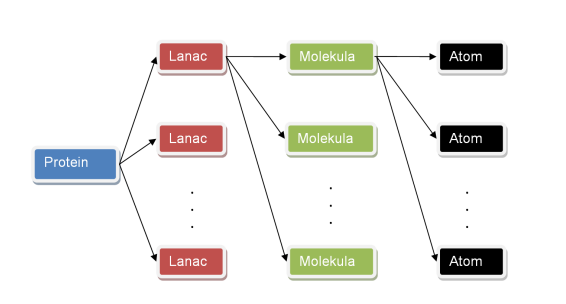
\includegraphics[width=5cm]{img/protein.png}
\caption{Struktura biomolekule}
\end{figure}

\subsection{Lanci u biomolekulama}
Proteinski lanci su složeni molekularni strukturi sastavljeni od aminokiselina, koje su manje gradivne jedinice. Atomi, najmanje strukturne jedinice proteina, igraju ključnu ulogu u njihovoj funkciji. U ovom kontekstu, posebnu važnost imaju metali i atomi koji djeluju kao donori elektrona. Donori su atomi kisika (O), dušika (N), klorida (Cl) i sumpora (S) koji se nalaze blizu metala na udaljenosti manjoj od 3 angstrema. Donori su negativno nabijeni i "doniraju" svoje elektrone metalima kako bi se postigla električna neutralnost. U svrh ovoga rada prepoznajemo ove vrste.
 \begin{enumerate}
  \item voda
  \item metali
  \item nukleinske kiseline (DNA i RNA)
   \item proteinski lanci
  \item ligandi (ostali)
  \end{enumerate}

  \begin{description}
   \item[Voda ] predstavlja lanac koji se sastoji od niza molekula vode. Sadrži jednu grupu atoma (HOH)
   \item[Metali ] predstavljaju jedan atom metal Fokusirat ćemo se na sljedeće metale: \linebreak
  		   Mg,Mn,Ni,Mo,Pt, Zn,K,Hg,Ba,Pb, 
		   Ca,Sr,Co,Al,V,Fe,Cu,W,Tl,Yb,Na,
                        Cd,Os,Au,Sm
   \item[Nukleinske kiseline ] su definirane kao lanci koji se sastoje od 90\% molekula iz sljedećeg  skupa DA,DT,DG,DC,DU,A,T,G,C,U

   \item[Proteinski lanci ]  su definirani duljine 50 molekula i sastavljeni su od 90\% molekula iz ovih aminokiselina
			       ALA,GLU,LEU,SER,ARG,GLN,LYS,THR,ASN,GLY \linebreak
                                       MET,TRP,ASP,HIS,PHE,TYR,CYS,ILE,PRO,VAL

   \item[Ligandi ]  su definirani kao lanci koji ne pripadaju u niti jednu gore navedenu skupinu.
  \end{description}

\chapter{Postojeći sustavi za analizu biomolekula}
 U istraživanju biomolekula, postoji niz softverskih alata koji omogućuju vizualizaciju i analizu struktura, interakcija i svojstava molekula.
 Ovi alati igraju ključnu ulogu u razumijevanju funkcionalnih aspekata biomolekula te pomažu u istraživanju njihove strukture i dinamike. 
 U nastavku su navedeni neki od popularnih sustava za analizu biomolekula koji su široko korišteni u znanstvenim istraživanjima.

PyMOL \cite{pymol} je jedan od najpoznatijih sustava za analizu biomolekula koji pruža napredne mogućnosti vizualizacije i interaktivne manipulacije biomolekula. 
On omogućuje detaljan pregled struktura, analizu interakcija i generiranje statistika. Također podržava Python skriptiranje, što omogućuje prilagodbu i automatizaciju analitičkih postupaka.

VMD (Visual Molecular Dynamics) \cite{vmd} kombinira vizualizaciju i analizu biomolekula. 
Pruža alate za prikazivanje struktura, analizu dinamike, generiranje animacija te analizu površina i vezanja liganda.
 Integracija s drugim softverskim paketima omogućuje daljnju analizu i obradu podataka.


MEPSUS (Metal Sites in Proteins Uniformly Sampled)  \cite{mepsus} je baza podataka koja se fokusira na geometriju vezanih metala u proteinima.
 Pruža informacije o distribuciji atoma prema koordinacijskim brojevima i kombinacijama aminokiselina koje sudjeluju u koordinaciji.
 MEPSUS omogućuje izradu statistika i analizu veza prema više molekula.

BioMe \cite{rakipovic} je napredni bioinformatički alat koji se fokusira na analizu metalo-proteinskih sustava. Jedna od glavnih prednosti BioMe alata je veliki broj statistika koje nudi, što ga čini jedinstvenim u odnosu na druge alate. 
BioMe također se ističe kao jedini alat koji omogućuje preuzimanje cjelokupne baze podataka, čime korisnicima omogućuje samostalno provođenje vlastitih statističkih analiza.
Sustav redovito ažurira svoje podatke, kako bi korisnicima pružao najnovije informacije, a istovremeno je jednostavan za proširenje i potpuno automatiziran.
Sustav je dostupan na \url{http://metals.zesoi.fer.hr}, no nažalost računanje statistika nije dostupno, zbog nepoznatog razloga.

Naposljetku ovaj rad je jedan od primjera takvih sustava, koji je nalik sustavu BioMe, naprednog alata za analizu metalo-proteinskih sustava.
Cilj ovoga rada je pružiti iste funkcionalnosti kao i stari sustav, uključujući veliki broj statistika.
Sustav je temeljena na najnovijim informacijama i pruža jednostavno proširiv i potpuno automatiziran okvir za analizu biomolekula. 
Kroz ovu repliku, željeli smo poboljšati prethodne nedostatke i ponuditi korisnicima snažan alat za njihova istraživanja u području metalo-proteinskih sustava.

\chapter{Arhitektura sustava}
 \textit{Arhitektura sustava može se podijeliti  na četiri podsustava: }

              \begin{enumerate}
               \item  Web  preglednik
                \item   Web aplikacija
	      \item   Parser podataka
                \item    Baza Podataka
                \end{enumerate}
	      \begin{figure}
                     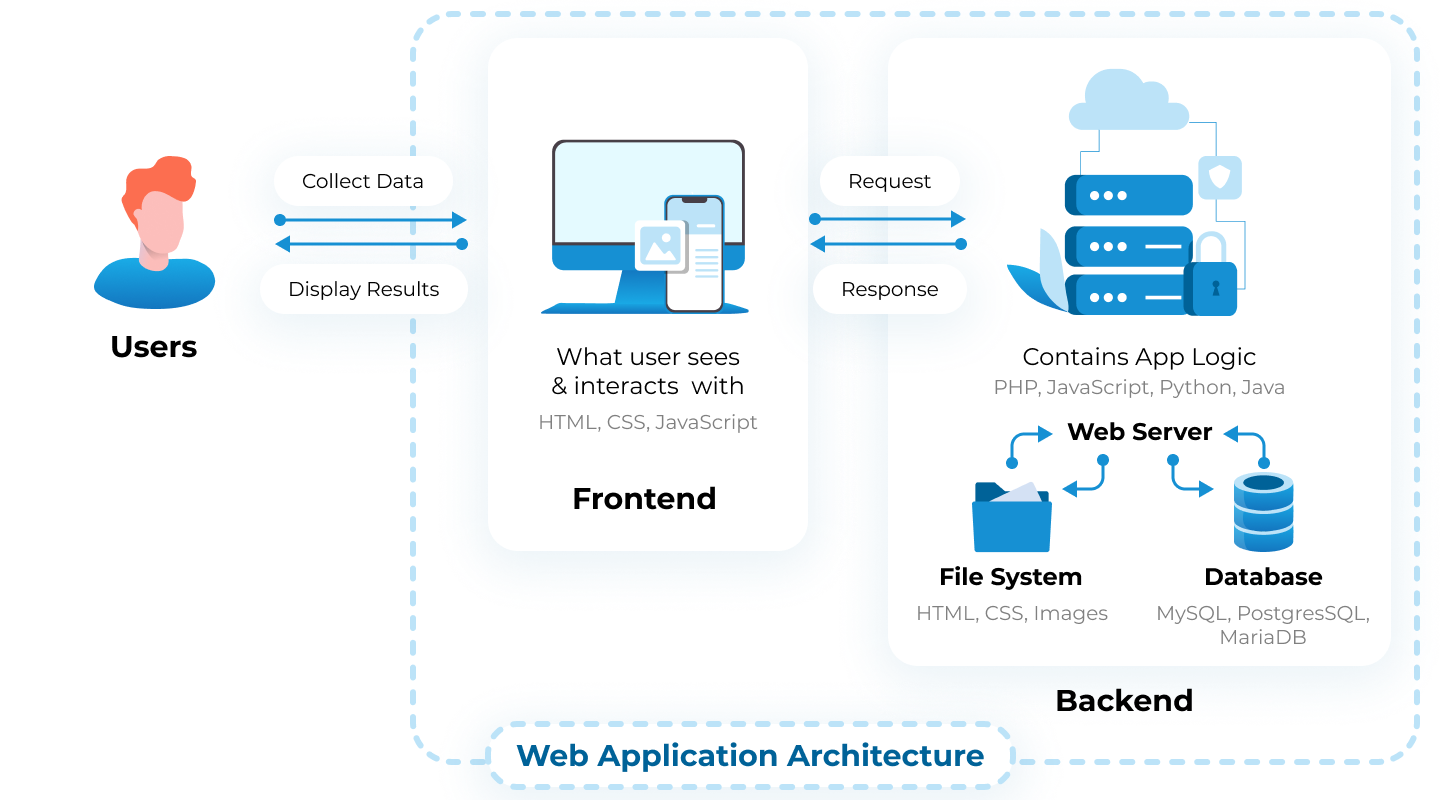
\includegraphics[width=7cm, height=5cm ]{./img/arhitektura.png}
                      \centering
                      \caption{Arhitektura sustava}
                  \end{figure}
	
\section{Web preglednik i poslužitelj}
Web preglednik i web poslužitelj su ključni sastavnici koji omogućuju funkcioniranje interneta putem HTTP(engl. Hypertext Transfer Protocol) protokola.

Web preglednik, kao softverska aplikacija, omogućuje korisnicima pregledavanje web stranica i pristupanje internetskim sadržajima koristeći HTTP protokol.
 Pomoću web preglednika korisnici mogu unijeti URL adrese web stranica, pretraživati internet.
 Primjeri popularnih web preglednika koji podržavaju HTTP su Google Chrome, Mozilla Firefox, Microsoft Edge, Safari i Opera.

Web poslužitelj, s druge strane, je računalni sustav ili program koji koristi HTTP protokol za pohranjivanje i dostavljanje web stranica korisnicima.
 Kada web preglednik šalje HTTP zahtjev, web poslužitelj prima taj zahtjev i obrađuje ga.
 Web poslužitelj pronalazi tražene datoteke koje čine web stranicu i šalje ih natrag web pregledniku putem HTTP odgovora.
 Ovaj odgovor sadrži statusni kod, sadržaj web stranice i druge relevantne informacije.

Dakle, HTTP protokol omogućuje komunikaciju između web preglednika i web poslužitelja. Web preglednik koristi HTTP za slanje zahtjeva web poslužitelju, dok web poslužitelj koristi HTTP za dostavljanje traženih datoteka i informacija web pregledniku.
 
\section{Web aplikacija}
Web aplikacija se obično sastoji od dvije ključne komponente: backend (poslužiteljska strana) i frontend (klijentska strana). Ove komponente zajedno čine arhitekturu web aplikacije.

Backend je dio web aplikacije koji se izvršava na web poslužitelju. On je odgovoran za obradu zahtjeva korisnika, manipulaciju podacima, poslovnu logiku i komunikaciju s bazom podataka. Backend koristi različite jezike programiranja i okvire (frameworks) poput PHP, Python, .Net , Java, Node.js itd. za izgradnju poslužiteljske logike.

Frontend je dio web aplikacije koji se izvršava na korisnikovom uređaju (npr. web pregledniku). To je korisničko sučelje s kojim korisnici interagiraju kako bi pristupili funkcionalnostima web aplikacije. Frontend koristi jezike kao što su HTML (Hypertext Markup Language), CSS (Cascading Style Sheets) za izgradnju funkcionalnosti web aplikacija.  Moderne frontend tehnologije i okviri poput React, Angular i Vue.js omogućuju razvoj kompleksnih i interaktivnih korisničkih sučelja.

Arhitektura web aplikacije omogućuje odvojenost poslovne logike, podataka i korisničkog sučelja. Backend se bavi poslovnom logikom i interakcijom s bazom podataka, dok frontend pruža korisničko sučelje i interakciju s korisnicima.

\section{Parser podataka}
Parser je podsustav koji obrađuje njemu predane mu mmCIF datoteke, provodi analize nad njezinim sadržajem i parsira u strukture koje se spremaju u bazu podataka.

Sustav je ključan za funkcioniranje web aplikacije, zbog konstantnog punjenja baze podataka najnovijim podatcima. Implementacija ovog sustava je preuzeta od 
studenta, koji ga je izradio u svom radu \cite{alanTus2010}. Sustav je implementiran u programskom jeziku java, koristeći biblioteku BioJava za parsiranje .cif podataka u
strukture, odnosno java objekte iz kojih radi razne analize, poput analizu udaljenosti. Svaka .cif datoteka se obrađuje posebno i završi sa spremanjem entiteta u bazu podataka. Ključna funkcionalnost sustava je konstantno skidanje najnovijih podataka, parsiranje i punjenje baze podataka. Koristi se Mysql baza podataka, a baza je
strukturirana kroz 5 entiteta. Sustav nažalost nije u funkciji, zbog zastarjele verzije biblioteke BioJava 1.7.1, te nije u mogućnosti pružati funkcionalnosti kako su zamišljene. U nastavku ćemo opisati korištenu biblioteku, strukturu baze, te izmjene koje su napravljene u ovome radu, kako bi sustav proradio.

\subsection{BioJava}
BioJava je biblioteka otvorenog koda (open-source) napisana u programskom jeziku Java koja pruža skup alata i funkcionalnosti za bioinformatičku analizu i manipulaciju bioloških podataka. BioJava je namijenjen prvenstveno za razvoj bioinformatičkih aplikacija i istraživanje u području biologije.

BioJava biblioteka pruža bogat set klasa i metoda za rad s različitim biološkim podacima kao što su sekvence DNA, RNA i proteina, strukturni podaci, genetski podaci, filogenetska stabla i drugi biološki entiteti. Također pruža funkcionalnosti za izvoz i uvoz podataka u standardiziranim formatima poput PDB, MMCIF i drugih. \cite{biojava}

BioJava također podržava razne bioinformatičke algoritme i metode za analizu sekvenci, poput poravnanja, pretrage, identifikacije i analize svojstava proteina. 

Formirajući Mavenov projekt unutar stare verzije projekta, ponudio je funkcionalnosti direktno korištenje najnovije verzije biblioteke.
Preuzimanjem biblioteke preko Maven repozitorija, omogućeno je lagano korištene novih metoda i razreda, kao da smo ih sami napisali.
Kompleksnost novije verzije, odnosno rasporeda informacija koje se nalaze u različitim razredima  uzrokovalo je probleme. 
Problemi su riješeni temeljitim proučavanjem biblioteke i primjenjivanjem primjera iz dokumentacije BioJave.
\subsection{MMCIF}
MMCIF (macromolecular Crystallographic Information File) je standardni format datoteke koji se koristi za pohranjivanje i razmjenu podataka o strukturi makromolekula, posebno proteina, dobivenih kroz kristalografske metode. Ovaj format se koristi u području strukturne biologije kako bi se opisale strukture proteina i njihovi detaljni podaci.
MMCIF datoteke su tekstualne datoteke koje sadrže informacije o atomima, vezama, kristalnoj rešetki, kristalnoj simetriji, kristalnim parametrima, eksperimentalnim metodama, rezoluciji i drugim relevantnim podacima o strukturi proteina. Format MMCIF koristi strukturiranu sintaksu za organiziranje i opisivanje podataka u obliku parova ključ-vrijednost.
Ovaj format je razvijen kako bi zamijenio stariji format PDB (Protein Data Bank), koji je bio manje strukturiran i ograničen u smislu podrške složenijim podacima o strukturi. MMCIF format pruža fleksibilnost za opisivanje različitih aspekata strukture proteina, kao i povezanih podataka kao što su eksperimentalni rezultati, vezanje liganda i slično.
\subsection{Cron}
Cron je standardni program koji se koristi u Unix i Unix-sličnim operativnim sustavima za automatsko izvršavanje zadataka u određeno vrijeme, periodički ili prema unaprijed definiranim rasporedima. 
Raspored izvršavanja zadatka u cronu definira se pomoću posebnog sintaksnog obrasca koji se sastoji od pet polja: minute, sati, dana u mjesecu, mjesec i dan u tjednu. Korisnik može navesti vrijednosti za svako polje kako bi odredio točno vrijeme izvršavanja zadatka. Cron je moćan alat za automatizaciju ponavljajućih zadataka i omogućuje korisnicima da učinkovito planiraju i upravljaju svojim zadacima bez potrebe za stalnim ručnim pokretanjem.

Parser podataka se pokreće kroz cron proces i obavlja iduće zadatke.

 	\begin{enumerate}
               \item  Sinkroniziranje s poslužiteljem za skidanje .cif datoteka
                \item   Arhiviranje starije verzije baze podataka
	      \item   Brisanje podataka iz baze
                \item    Pokretanje parsera
                \end{enumerate}
U ovom dijelu sustava, ovaj rad nije ništa mijenjao, ali je korišten za tesitranje pri popravku starije verzije parsera.

\section{Baza podataka}
  Baza podataka je organizirana kolekcija podataka koja omogućuje skladištenje, upravljanje i manipulaciju podacima. Ona se koristi za pohranjivanje strukturiranih  podataka kao što su tekst, brojevi, slike ili druge vrste informacija.
Baze podataka omogućuju učinkovito upravljanje velikim količinama podataka i omogućuju pristup tim podacima putem različitih aplikacija.

 BioMe sustava (Rakipović 2012.), koristi MySQL bazu podataka, koja je preuzeta od sustava parsiranja (Tus 2010.) jer je tada bila najbolja besplatna relacijska baza. U ovome radu baza podataka je prebačena na PostgreSQL, koja je trenutačno najbolja besplatna relacijska baza. Struktura baze preuzeta je iz rada
Tusa, a ima ovakvu strukturu. Pdb relacija nudi informacije  o svim strukturama uz atribute oznaka strukture, naziv, rezolucija.
 Na pdb relaciju veže se chain relacija, koja sadrži informacije o lancima  od kojih se sastoji struktura proteina. 
Relacija chain vezana je s relacijama residue i atom. Residue relacija pruža podatke o grupama atoma koje sačinjavaju lance.
 Relacija atom u sebi ima podatke o korištenim atomima u strukturama.
 Atom ima atribute oznaku atoma,strukture,lanca i grupe atoma kojemu pripada.
 Relacije angle i distance se vežu na relaciju atoma, te sadrže podatke o kutovima između atoma donora i udaljenosti između atoma metala.

Migracija iz MySQL u PostgreSQL bazu je ostvarena, tako što je  datoteka s opisom stare baze, prevedena u komande druge baze, te pri izvršenjem skripte 
stvorena je prazna baza. Naknadno se samo u novoj implementaciji parsera, promijenio Jdbc driver iz mysql u Postgres, kako bi se baza mogla napuniti podatcima.
\subsection{PostgreSql}
PostgreSQL je napredni objektno-relacijski sustav za upravljanje bazama podataka otvorenog koda. On podržava kompleksne podatke i prilagođene tipove, te omogućuje proširivost i prilagodbu bazi podataka. PostgreSQL ima ACID svojstva transakcija i napredne mehanizme za prikupljanje statističkih podataka. Također podržava replikaciju i visoku dostupnost te koristi moćan SQL upitni jezik. Kao popularan izbor za razne aplikacije, PostgreSQL ima aktivnu zajednicu koja pruža podršku i kontinuirano razvija sustav.  \cite{postgresql}

\section{MVC}
  MVC (Model-View-Controller) je arhitekturalni obrazac koji se često koristi u razvoju softvera, posebno za razvoj web aplikacija. Ova arhitektura pomaže u organizaciji koda, poboljšava održivost i olakšava timski rad.

MVC arhitektura se sastoji od tri osnovne komponente:

\begin{description}
  \item[Model (Model)] : Model predstavlja strukturu podataka i poslovnu logiku aplikacije. Ovdje se nalaze podaci s kojima aplikacija radi, kao i metode za pristup, manipulaciju i ažuriranje tih podataka. Model ne zna ništa o korisničkom sučelju ili prikazu podataka, već se fokusira samo na obradu podataka.
  
   \item[Pogled (View)] :   Pogled predstavlja korisničko sučelje vaše aplikacije. Pogled ne sadrži poslovnu logiku, već samo prikazuje podatke koje dobiva od Modela. Pogled može biti oblikovan kao HTML stranica, korisnički widget ili bilo koji drugi način prikaza podataka.
 
   \item[Kontroler (Controller)] :  Kontroler je posrednik između Modela i Pogleda. On prima korisnički unos ili događaje s Pogleda i obrađuje ih. Kontroler komunicira s Modelom kako bi dohvatio ili ažurirao podatke te zatim obavještava Pogled o rezultatima. Kontroler također može obavljati dodatne zadatke kao što je validacija unosa ili upravljanje tijekom aplikacije.
\end{description}

MVC arhitektura je postala vrlo popularna u razvoju web aplikacija jer omogućava efikasno razdvajanje odgovornosti između front-end i back-end dijelova aplikacije. 


  \begin{figure}[!htb]
	\centering
	\hspace*{-2.5cm}
	 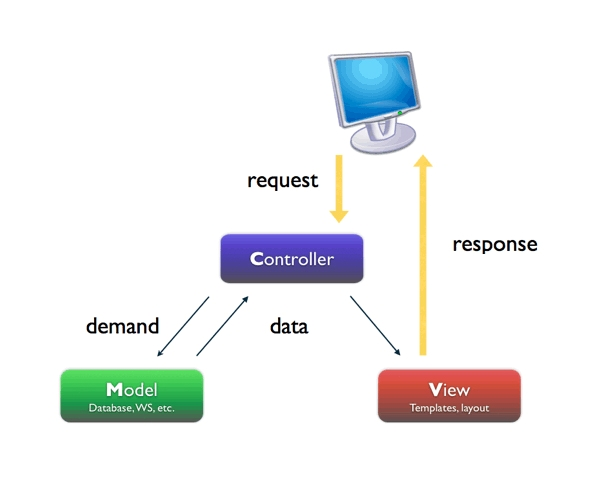
\includegraphics[width=\dimexpr\paperwidth-10cm,height=\dimexpr\paperheight-15cm,keepaspectratio]
	{./img/mvc.jpg}
		\centering
                      \caption{MVC model}
    \end{figure}


   \begin{figure}[!htb]
	\centering
	\hspace*{-2.5cm}
	 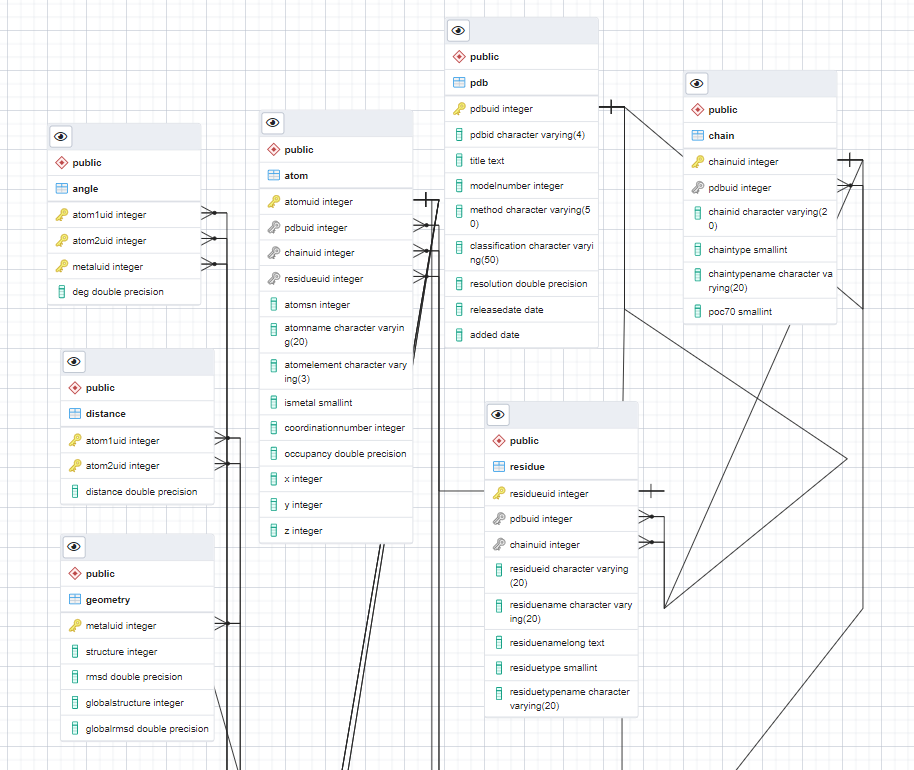
\includegraphics[width=\dimexpr\paperwidth-2cm,height=\paperheight,keepaspectratio]
	{./img/ERdijagram.png}
		\centering
                      \caption{ER dijagram baze podataka.}
    \end{figure}

\chapter{Implementacija}
\section{Frontend}
 Korisničko sučelje implementirano je u tehnologiji Angular 15 u razvojnom okruženju (engl. IDE) Visual Studio Code. Dodatno je korištena tehnologija bootstrap 5
radi lakšeg pisanja CSS datoteci i bržeg razvijanja sučelja. \cite{angular}

 Angular je open-source framework razvijen od strane Googlea, koji se koristi za izgradnju robusnih, skalabilnih i dinamičnih web aplikacija. 
Angular koristi TypeScript, nadskup JavaScripta, kao svoj glavni jezik za pisanje koda. TypeScript donosi prednosti statičke tipizacije, bolje otkrivanje grešaka i razumijevanje koda. Ovo pomaže programerima da lakše razvijaju i održavaju kompleksne aplikacije.

Primjerak aplikacije stvara se ovom naredbom: 
\begin{lstlisting}[language=bash]
   $ ng new Frontend
\end{lstlisting}
 
\subsection{Angular Komponente}
Temeljna jedinica za izradu sučelja su komponente. Angular komponente sastoje se od 3 osnova dijela : 
Predložak (engl. Template) : HTML kod koji definira izgled komponente i koristi se za interakciju s korisnikom.
Klasa komponente (engl. Component Class) : TypeScript klasa koja definira logiku komponente.
Stilovi (engl. Styles) : CSS kod koji definira boje,fontove i raspored komponenata

\subsection{Bootstrap}
Bootstrap je open-source framework za razvoj web aplikacija. Pruža alate, stilove i predloške za izradu modernih, responzivnih korisničkih sučelja. Omogućava brzo izgraditi web stranice prilagođene različitim uređajima. 
Uključuje gotove stilove, komponente i responzivnu rešetku. Ovu  moćnu tehnologiju lagano možemo ukomponirati u svoju aplikaciju s ovom komandom.

\begin{lstlisting}[language= bash]
   $ npm install bootstrap --save
\end{lstlisting}

\section{Backend}
Pozadinski dio aplikacije implementiran je u .NET razvojnom okviru (engl. framework) koristeći razvojno okruženje Visual Studio. Umjesto ručnog pisanja SQL upita prema bazi podataka,  \cite{dotnet}
korišten je primjerak ORM-a (Object Relation Model) Entity Framework, koji nam omogućuje lakše operiranje s bazom podataka.

.NET Framework pruža skup alata, biblioteka i tehnologija za razvoj različitih vrsta aplikacija, uključujući web aplikacije, desktop aplikacije, mobilne aplikacije, usluge i još mnogo toga.

S obzirom na to da je .NET Framework razvijen od strane Microsofta, on ima snažnu podršku, dobru dokumentaciju i aktivnu zajednicu razvojnih programera. Također pruža alate za razvoj, testiranje, implementaciju i održavanje aplikacija.

\subsection{Controller i Service}
Temeljni dijelovi pozadinskog dijela aplikacije su kontroleri. Kontroler su C\# klase, koji ima niz metoda  koje se odnose na specifične operacije koje treba izvršiti.
Takve operacije se označavaju atributima poput "HttpGet" , "HttpPost" itd, koji određuju koju će HTTP metodu upotrijebiti u akciji.

Kontroleri u .NET-u obično koriste usluge (services) i repozitorije za pristup podacima i izvršavanje poslovne logike. Ovo promiče princip razdvajanja odgovornosti (engl. Separation of Concerns) i olakšava testiranje i održavanje aplikacije. 

\subsection{Entity Framework}
Entity Framework (EF) je ORM (Object-Relational Mapping) alat koji je dio .NET Frameworka. On omogućava programerima da rade s podacima iz baze podataka kao objektima, koristeći objektno-orijentirane koncepte, umjesto da rukovode niskim pristupom  SQL upitima i ručnim mapiranjem podataka. \cite{ef}

Glavna svrha Entity Frameworka je olakšavanje interakcije s bazom podataka putem jednostavnog i intuitivnog objektnog modela. Programeri mogu definirati entitete, odnosno klase koje predstavljaju tablice u bazi podataka, i mapirati ih na odgovarajuće tablice.

\section{Tehnologija Git}
Git je distribuirani sustav za upravljanje verzijama softverskog koda. Omogućava praćenje promjena, suradnju, grananje i spajanje kodova. Sadrži lokalne repozitorije za rad bez stalne mrežne veze i podršku za suradnički rad. Ova tehnologija korištena je  radi samoprovjere napretka u implementaciji sustava. 
\cite{git}

\section{Opis sustava}
 \subsection{Korisničko sučelje}

Korisničko sučelje implementirano je s 2 pogleda Dashboard i Statistics.

Dashboard stranica sadrži veliku formu za unos parametara pretrage i statističkih parametara. Ova stranica je implementirana s 7 komponenti.

Dashboard komponenta je centralna komponenta, koja sadrži u sebi sve ostale komponente i zadužena je za prikupljanje podataka od ostalih 6 komponenti
nakon pritiska na gumb Submit.

Statistic Scope komponenta je komponenta zadužena za prikupljanje informacija o razini pdb pretraživanja. Komponenta pruža opciju pretraživanja prema jednom pdb,
više njih i sve pdb, koje sustav trenutno ima u bazi podataka.

Method Filter komponenta je zadužena za odabir metode preko koje su pronađeni određeni atomi metala. Nudi opciju bilo koje metode, NMR metode i XRAY metode, no
uz odabir XRAY metode mora se navesti rezolucija (engl. resolution).

Geometry komponenta je zadužena za odabir 3 stvari udaljenosti između metala, koordinacijskog broja I RMSD. Ako korisnik ne odabere ništa, za udaljenost će se uzeti
broj 7, koordinacijski broj će biti 1, a RMSD će biti 15.

Metals komponenta je zadužena za odabir metala nad kojima će se voditi pretraga ili izračun statistike. Komponenta nam nudi 25 mogućih metala, koji su navedeni u sekciji 
2.4.1 ovog rada. Osim toga, radi lakšeg odabira svih metala dodan je gumb s kojim se automatski mogu odabrati svi metali  pritiskom na gumb  Toggle.

Ligands komponenta je slična komponenti Metals, no u njoj se biraju ligandi, koji će biti uključeni u pretragu ili izračun statistike. Komponenta nudi automatsko biranje
Amino kiselina pritiskom na gumb Toggle AA i odabir Nukleinskih kiselina pritiskom na gumb Toggle NA.

Chains komponenta je zadužena za odabir tip lanaca na koje će se fokusirati statistike. Nude nam 5 tipova lanaca : Proteinske, DNK,RNK, Vodu i druge.
Ovi tipovi lanaca su opisani u sekciji 2.4.1.

Pritiskom na gumb submit, odlazimo na stranicu Statistics.
Ova stranica je sačinjena od sedam  komponenata i zadužena je za prikaz izračunatih statistika.

Statistic komponenta je centralna komponenta, koja prikazuje svaku od ostalih komponenata. No nisu sve statistike odjednom prikazane. Pritiskom na link koji će prikazati izračunatu statistiku. 

Home komponenta  ima ulogu (engl. landing pagea), to je prva stvar koju vidite nakon pritiska gumba submit.

StatisticM1-M7 su komponente sadužene za izračun statistika M1-M7.

Statistike će objašnjenje kasnije.

Kako bi ovaj dio sustava funkcionirao potreban nam je nekakav razred (engl. class), koji će nam držati podatke što je korisnik unio. Zato imamo razred
StatisticDto, koji je ulazni parametar svih statistika. Primjerak takvog razreda šalje se na poslužiteljsku stranu 

  \begin{figure}[!htb]
	\centering
	\hspace*{-2.5cm}
	 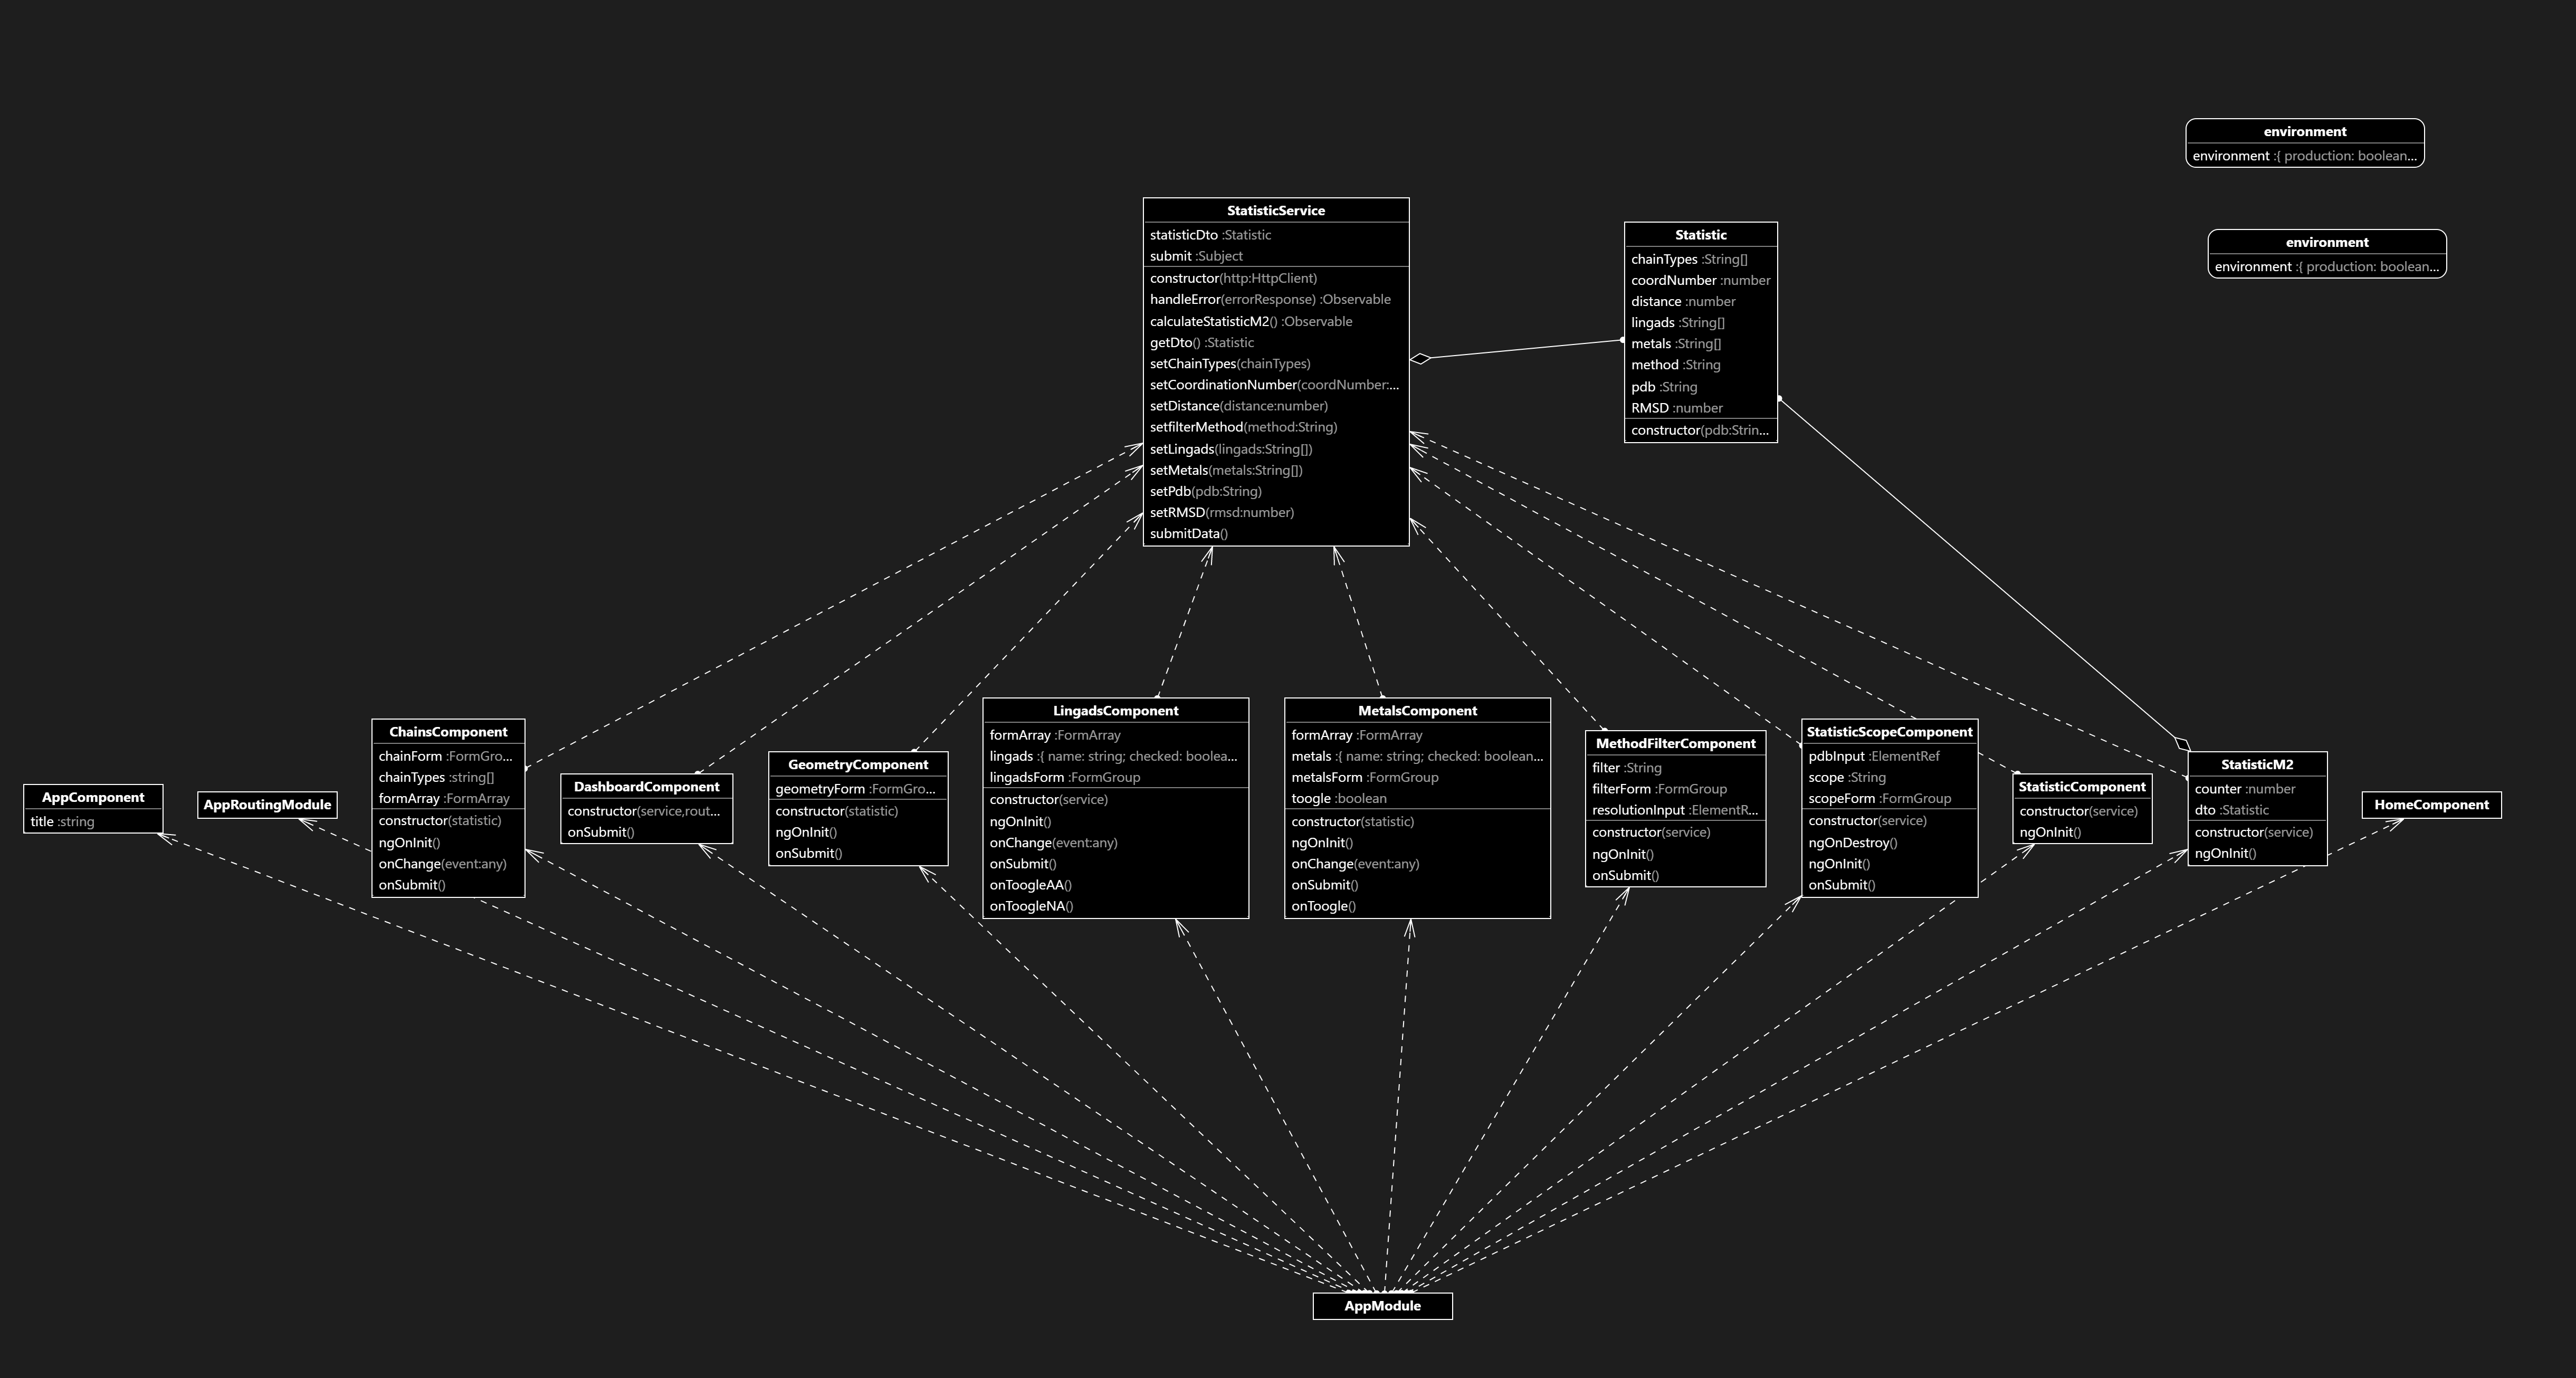
\includegraphics[width=22cm,height=\paperheight,keepaspectratio,angle=90]
	{./img/frontend.png}
		\centering
                      \caption{Dijagram razreda frontend.}
    \end{figure}

\subsection{Poslužiteljska strana}
Ovaj dio sustava implementiran je kroz jedan kontroler, dva servisa i 7 razreda.

Statistic Controller je razred koji predstavlja kontroler i odgovara na http zahtjeve od korisničkog sučelja. Sadrži 8 metoda vrsti HTTP-Post, svaka od njih predstavlja
jednu statistiku. 

IStatisticMService i StatisticMService predstavljaju jedan servise, koji računaju statistike vezane uz metale.

IStatisticLService i StatisticLService predstavljaju drugi servis, koji računa statistike vezane uz ligande.

Razredi Scope,Method,Distance,Geometry,Atom, Chain predstavljaju naše entitete u bazi podataka, preko kojih dohvaćamo redove iz tablica.

MetalsDbContext je centralni razred svih modela navedenih iznad. Preko njega biblioteka Entity-Framework zna s kojim entitetima on upravlja u bazi.
Kroz njega možemo definirati relacije između modela, odnosno entiteta u bazi, no u ovome radu je to implementirano kroz anotacije unutar samih modela.

StatisticDto je razred koji nam služi za prihvaćanje podataka odnosno njemu sličnog razreda iz  frontend dijela aplikacije.

  \begin{figure}[!htb]
	\centering
	\hspace*{-2.5cm}
	 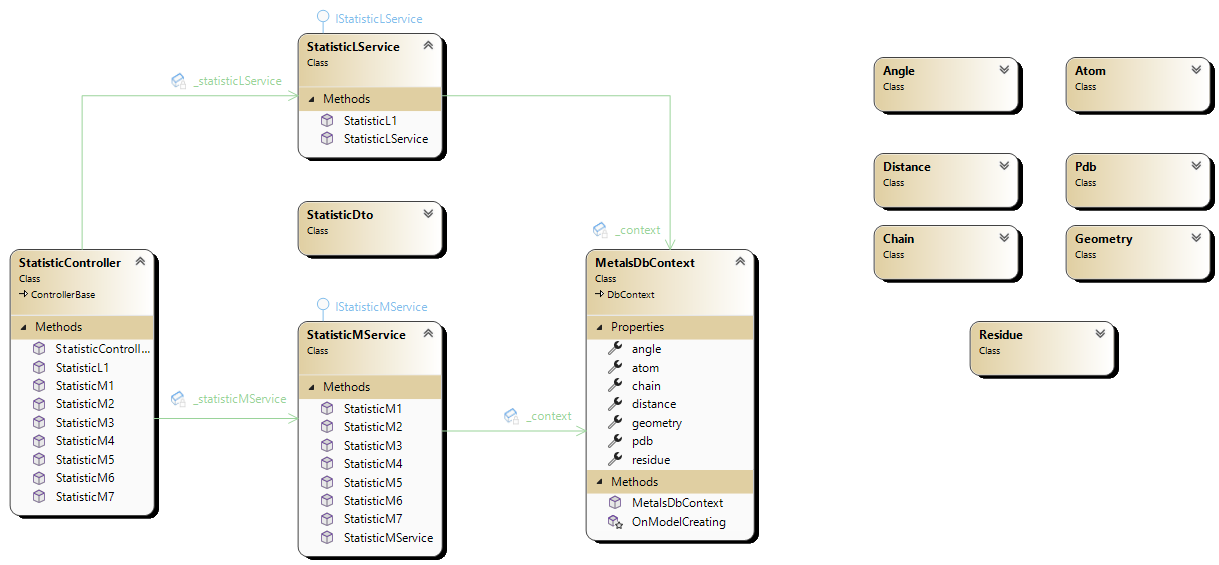
\includegraphics[width=\dimexpr\paperwidth-2cm,height=\paperheight,keepaspectratio]
	{./img/backend.png}
		\centering
                      \caption{Dijagram razreda Backend.}
    \end{figure}

\section{Funkcionalnosti}
U ovome poglavlju ćemo prikazati funkcionalnosti sustava, odnosno prikazat ćemo jedan primjer korištenja sustava.
Izračuni statistika nisu pouzdani, zbog ne stručnosti u izradi sustava.  Prikazane statistike bit će izračunate za određeni set parametara.
Odabrat ćemo metale Mg i Ca, te aminokiseline ASP I GLU s koordinacijskim brojem 4. Pretraživanje u bazi ćemo obavljati u skupu svih PDB-ova, a filtracijska metoda
će biti postavljena na bilo koju metodu. Udaljenost između metala bit će pretpostavljena, odnosno 7. Na slici ispod prikazan je prva stranica aplikacije, koja je jedan velika forma s mogućnosti odabira svih gore navedenih parametara. Kako bi parametri bili registrirani, nakon odabira mora se kliknuti gumb "OK".

  \begin{figure}[!htb]
	\centering
	\hspace*{-2.5cm}
	 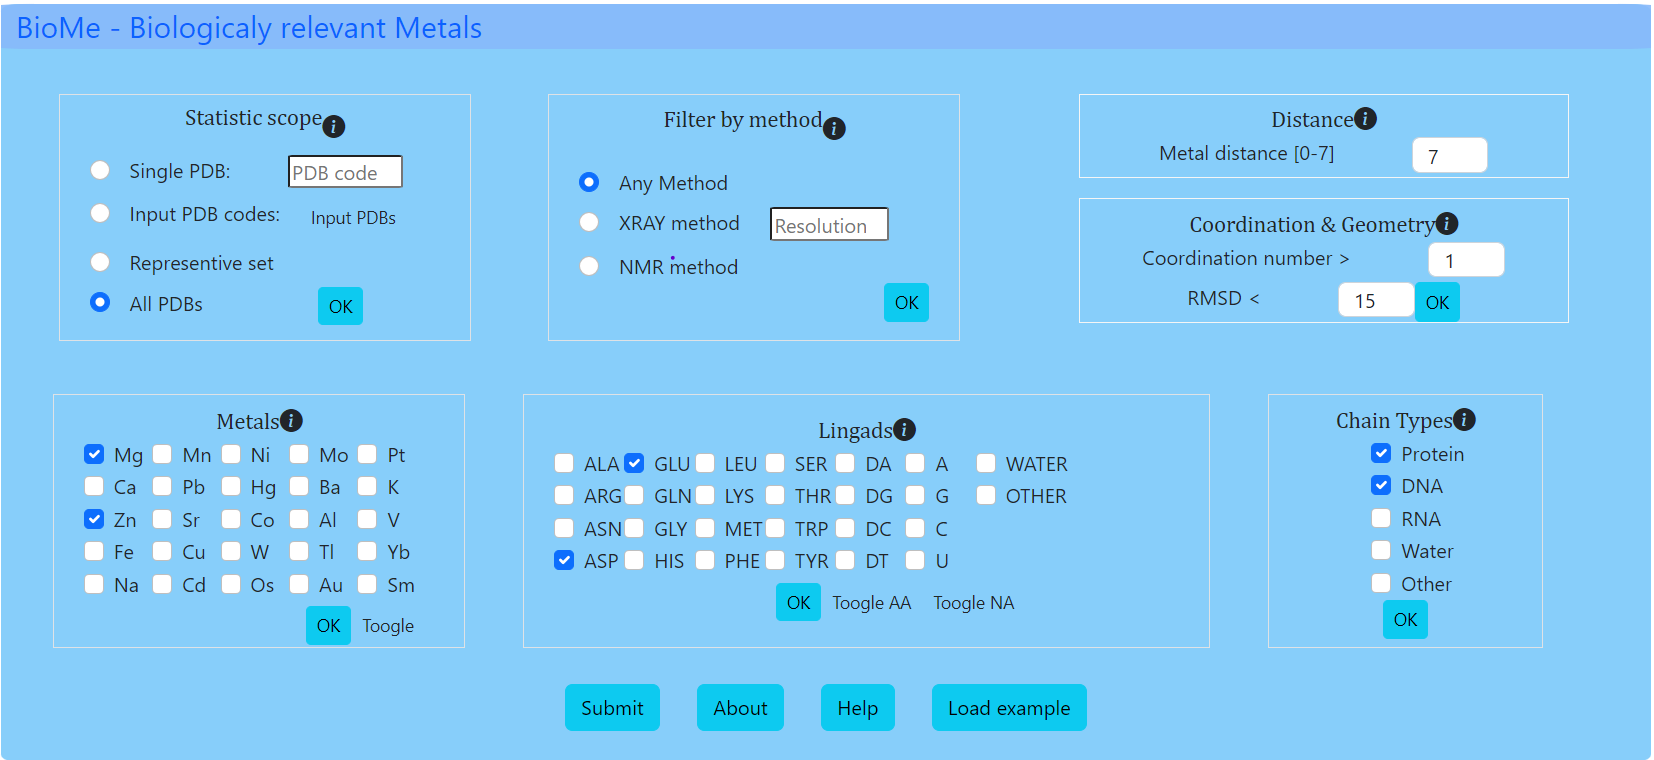
\includegraphics[width=\dimexpr\paperwidth-2cm,height=\paperheight,keepaspectratio]
	{./img/websucelje.png}
		\centering
                      \caption{Prikaz web sucelja.}
    \end{figure}

Nakon pritiska gumba "Submit" ili "Load example", koji će za vas izgenerirati ovaj primjer iznad. Dolazimo na drugu stranicu, odnosno stranicu sa statistikama
Pritiskom u zaglavlju na bilo koji gumb, dobiti ćemo izračune statistika. Postoji gumb "HOME", koji će vas vratiti na početnu stranicu statistika.

  \begin{figure}[!htb]
	\centering
	\hspace*{-2.5cm}
	 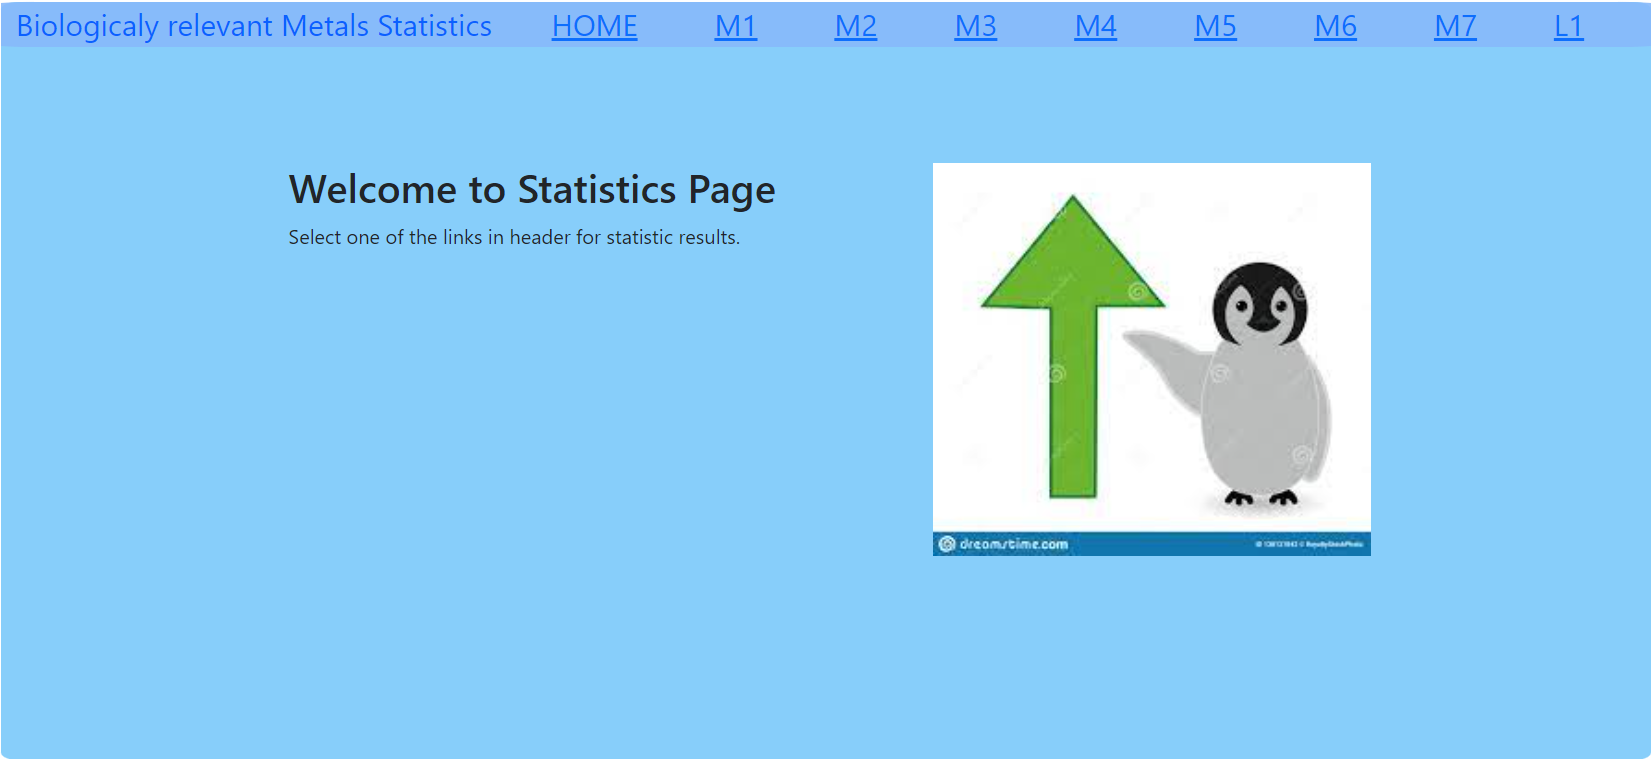
\includegraphics[width=\dimexpr\paperwidth-2cm,height=\paperheight,keepaspectratio]
	{./img/statistics.png}
		\centering
                      \caption{Prikaz Statistika.}
    \end{figure}

Sustav nudi dvije vrste statistika : (M1-M7) statistike koje se računaju za označene metale 
					 (L1) statistika koja se računa za označene ligande.

Sustav ne nudi implementaciju svih statistika, zbog već navedene ne stručnosti, no barem ćemo opisati što bi trebali raditi te statistike.

\subsection{M1 - Distribucija veza metala s odabranim ligandima}
M1 statistika prikazuje kako se atomi metala vežu na izabrane ligande.
Metal je u vezi s ligandom, ako je jedan atom metala udaljen za manje od 3 od bilo kojeg atoma ligada.
Broj veza računa se kao zbroj veza svih atoma tog metala s odabranim ligandom.

  \begin{figure}[!htb]
	\centering
	\hspace*{-2.5cm}
	 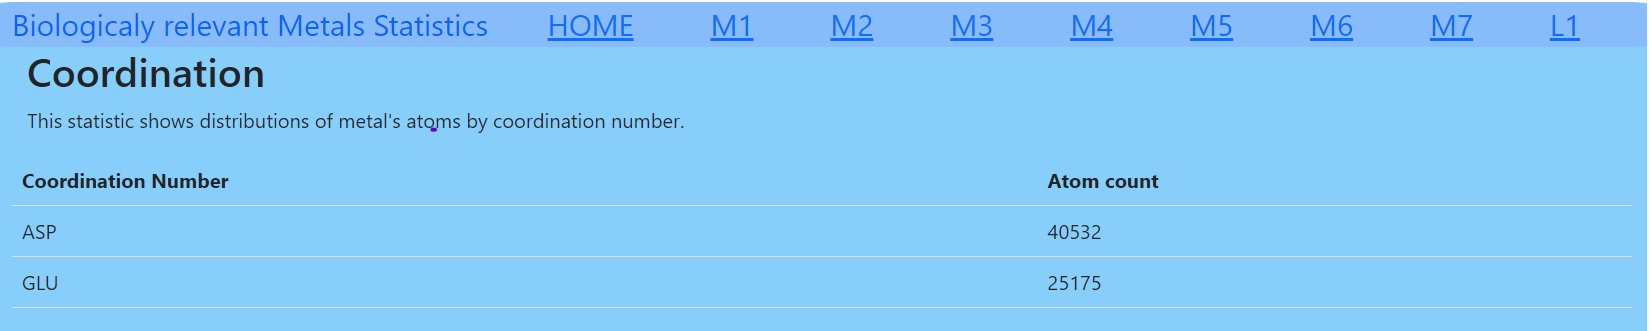
\includegraphics[width=\dimexpr\paperwidth-2cm,height=\paperheight,keepaspectratio]
	{./img/M1.png}
		\centering
                      \caption{Prikaz statistike M1.}
    \end{figure}


\subsection{M2 - Distribucija broja atoma metala po koordinacijskom broju }
Ova statistika računa broj atoma izabranog metala za određeni koordinacijski broj.
Statistika daje računa za jedan metal, no možete vi odabrati i njih više, ali će statistika izračunati samo za prvog kojeg ste izabrali.

\begin{figure}[!htb]
	\centering
	\hspace*{-2.5cm}
	 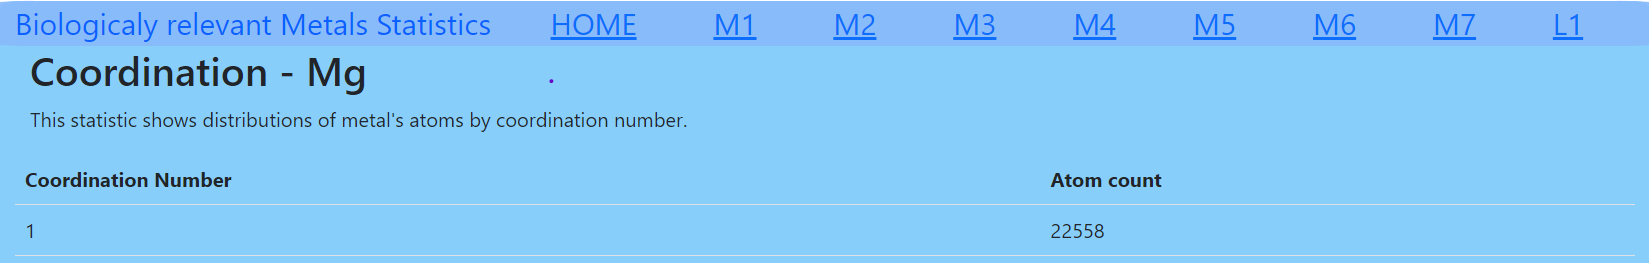
\includegraphics[width=\dimexpr\paperwidth-2cm,height=\paperheight,keepaspectratio]
	{./img/M2.png}
		\centering
                      \caption{Prikaz statistike M2.}
    \end{figure}

\subsection{M3 - Kombinacije lingada po koordinacijskom broju }
Za izračun ove statistike potrebno je odabrati koordinacijski broj.
Računa se broj kombinacija označenih lingada s pojedinim atomom metala.

Ova statistika nije implementirana, no u sustavu se može kliknuti na link, ali neće biti nikakvih rezultata.
Na slici ispod je prikazano, što će biti ispisano za neimplementirane statistike

\begin{figure}[!htb]
	\centering
	\hspace*{-2.5cm}
	 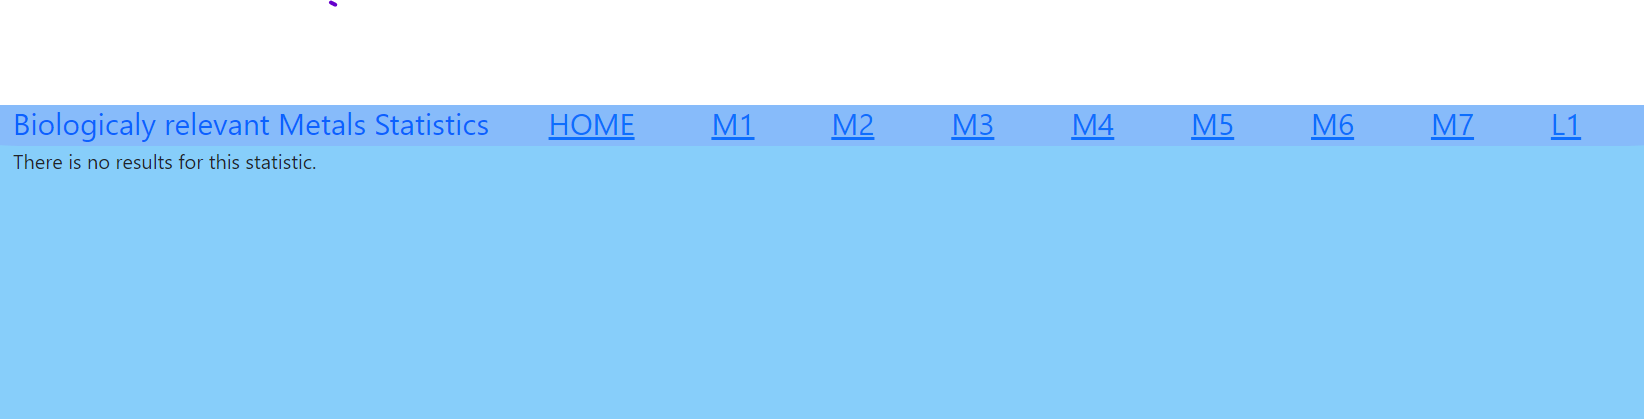
\includegraphics[width=\dimexpr\paperwidth-2cm,height=\paperheight,keepaspectratio]
	{./img/empty.png}
		\centering
                      \caption{Prikaz prazne statistike.}
    \end{figure}

\subsection{M4 - Distribucija monodentatno i bidentantno koordiniranih metala s ASP i GLU}
Statistika prikazuje broj monodentatno i bidentantno koordiniranih metala.

Statistika također nije izračunata.

\subsection{M5 - Distribucija atoma metala s atomima vezani za isti lanac}

\begin{figure}[!htb]
	\centering
	\hspace*{-2.5cm}
	 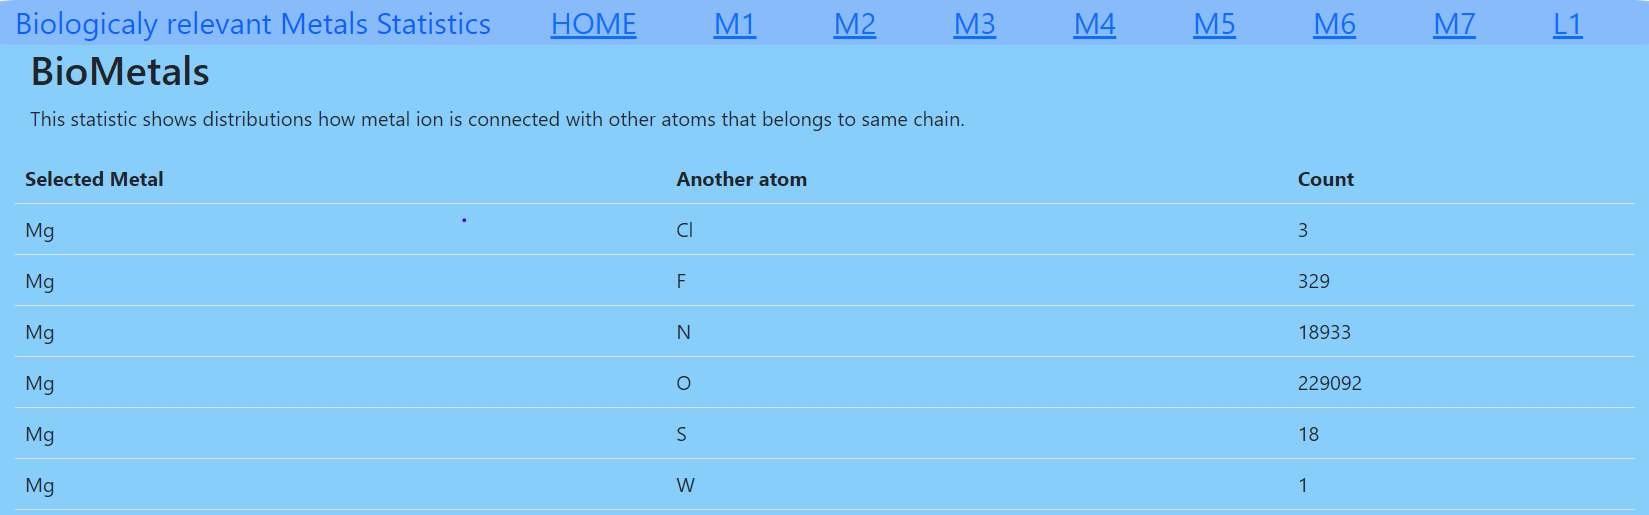
\includegraphics[width=\dimexpr\paperwidth-2cm,height=\paperheight,keepaspectratio]
	{./img/M5.png}
		\centering
                      \caption{Prikaz statistike M5.}
    \end{figure}

Statistika računa u broj atoma povezanih s odabranim metalom, koji se nalaze na istom lancu.
Atomi su povezani ako su udaljeni za manje od željene udaljenosti od bilo kojeg atoma tog metala. 
Udaljenost metala (engl. metal distance) može se odabrati u sučelju te nudi brojeve 0-7.

Također možete odabrati više metala u korisničkom sučelju, no ova statistika bit će izračunata, samo za prvi kojeg ste odabrali.
No, ako odaberete samo jedan, bit će izračunata za njega.


\subsection{M6 - Distribucija koordinacijske geometrije po metalima}
Statistika računa broj atoma metala u geometrijskoj strukturi s obzirom na parametar RMSD. RMSD označava srednju vrijednost devijacije od idealne geometrijske
strukture. Prikazuju se rezultati koji su ispod vrijednosti RMSD.

Statistika također nije implementirana.


\subsection{M7 - Srednja udaljenost i standardna devijacija udaljenosti metala}
Ova statistika pokazuje broj veza odabranog metala s nemetalima iz ovog skupa: Cl,O,S,F I N
Uz to statistika računa srednju vrijednost udaljenosti i standardnu devijaciju.

\begin{figure}[!htb]
	\centering
	\hspace*{-2.5cm}
	 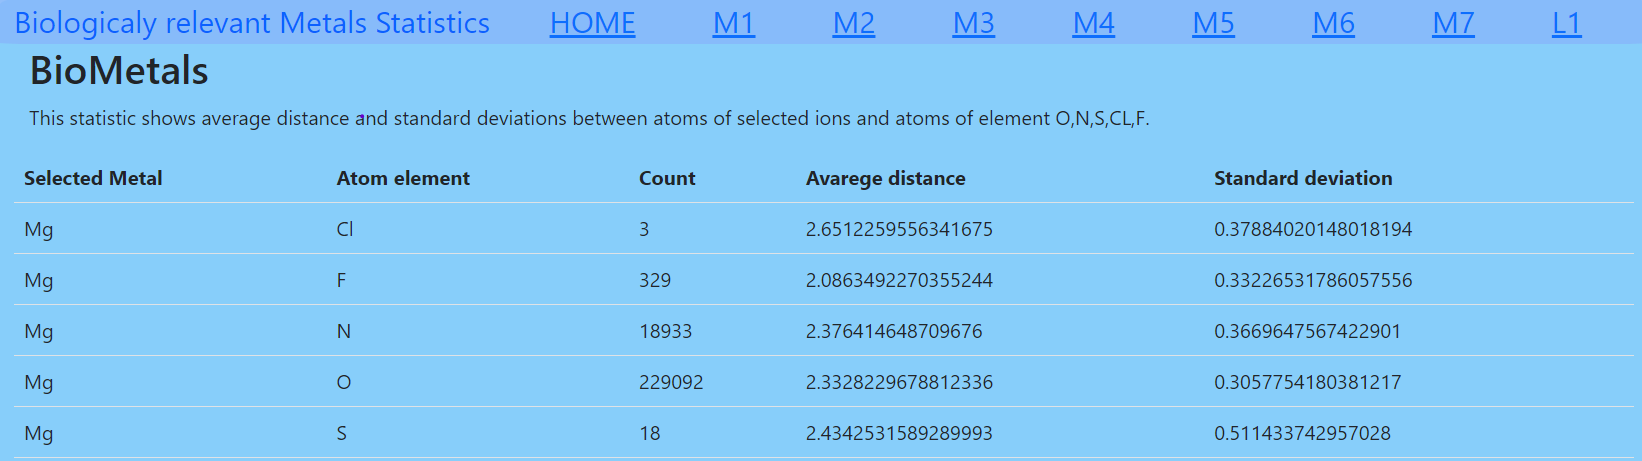
\includegraphics[width=\dimexpr\paperwidth-2cm,height=\paperheight,keepaspectratio]
	{./img/M7.png}
		\centering
                      \caption{Prikaz statistike M7.}
    \end{figure}

\subsection{L1 - Distribucija atoma metala po ligandima}
Statistika računa broj veza atoma  odabranih metala s odabranim ligandom.
Atom metala je u vezi s lingadom, ako je udaljen za manje od 3 od bilo kojeg atoma ligada.

Statistika također nije implementirana.

\chapter{Zaključak}
Sustav nam nudi razna pretraživanja i statistike vezane za odnose između metala i lingada.
Web aplikacija nudi pretragu s odabirom pet vrsti lanaca, dvadeset lingada i 25 metala.
Metali su iz odabranog skupa metala, dok su lingadi  podijeljeni na nukleinske i aminokiseline.
Uz to sustav nudi pretrage po pdb, filtraciju po metodi, te odabir raznih parametara za izračun statistika.
Primjer koji je opisan u ovome radu, je dostupan za isprobati u aplikaciji klikom na gumb Load Example.
Tipična primjena sustava započinje odabirom svih željenih parametara, nakon čega se može birati
koju statistiku želimo izvršiti. Statistike se dijele na dvije vrste: M I L, odnosno statistike koje se bave metalima i one koje se bave ligandima.

Cilj ovoga rada je ponovno upogoniti BioMe sustav. To je učinjeno poprilično dobro, no zbog manjka profesionalnosti u razumijevanju grane bioinformatike, pogotovo metala i njihovih među odnosa nisu implementirane sve statistike.
Replika BioMe sustava je implementirana u novijim tehnologijama i koristi potpuno drugu bazu podataka, što dovodi do bržeg i sigurnijeg rada sustava. Zbog naprednijih tehnologija, nisu se morale provoditi nikakvi optimizacijski algoritmi, kao
stvaranje privremene tablice ili smanjivanja broj SQL upita. Prednost replike Biome sustava, nad onim starim je što se statistike računaju, prema odabiru korisnika i ne sve odjednom, što dodatno smanjuje vrijeme čekanja na bilo kakve rezultate.
Kako bi ovaj sustav parirao raznim sustavima sirom svijeta, potreban je dodatan rad sa stručnjacima u sklopu nekog projekta, kako bi se utvrdile točni izračuni statistika.

\bibliography{literatura}

\bibliographystyle{fer}

\title{Web aplikacija za pretraživanje baze biološki značajnih metala}
\begin{sazetak}

Ovaj rad donosi opis sustava za analizu biomolekula, kroz pretraživanja i statistike.
Arhitektura sustava sastoji se od 3 dijela :  web aplikacija, parser podataka , baza podataka.
Prije razvitka web aplikacije, prvi na red su došli parser podataka i baza podataka.
Sustav koristi PostgreSQL bazu podataka, sa strukturom preuzetom iz rada Tus-a. Baza sadrži informacije o strukturama, lancima, ligandima i atomima, te udaljenostima između atoma, popraćeni s geometrijskim strukturama i kutovima.
Parser podataka je dio sustava, koji puni bazu podataka tim potrebnim informacijama.
Ključni dio sustava je web aplikacija  implementiran je kao dva pod sustava : Korisničko sučelje (engl. Fronted) i Pozadinska strana (engl. Backend).
Korisničko sučelje je implementirano u razvojnom okviru Angular 15, dok je Pozadinska strana implantirana u razvojnom okviru .Net. 
Kroz interakciju s web aplikacijom, korisnik može saznati razne informacije o metalima i njihovim međudjelovanjem s ligandima.
Takvi rezultati dostupni su nakon ispunjavanja forme, odnosno parametara koji će biti uključeni u izračun statistika.
Rezultati statistika su dostupni u tabličnom formatu.
Sustav u usporedbi s BioMe sustavom nije bolji, ali je ponovno upogonio ideju sustava Alena Rakipovića u duhu novih tehnologija.
Mane ovog sustava su nepouzdanost rezultata statistika i nemogućnost dohvaćanja svih statistika, jer nisu sve implementirane.

Sustav nije dostupan na internetu, no njegov kod potreban za pokretanje bit će dostupan na ovome linku, osobnog GitHub računa.

\kljucnerijeci{biomolekule,metali,lingadi,nukleinske kiseline,frontend,backend,statistike}
\end{sazetak}

% TODO: Navedite naslov na engleskom jeziku.
\engtitle{A web application for searching biologicaly relevant metals database}
\begin{abstract}
This paper presents a description of a biomolecular analysis system that utilizes search and statistical techniques. The system architecture consists of three components: a web application, a data parser, and a database. Prior to developing the web application, the data parser and database were implemented. The system utilizes a PostgreSQL database with a structure adapted from the Tus paper, containing information about structures, chains, ligands, atoms, as well as distances between atoms accompanied by geometric structures and angles.

The data parser is an integral part of the system, responsible for populating the database with the necessary information. The key component of the system is the web application, which is implemented as two subsystems: the Frontend, developed using the Angular 15 framework, and the Backend, developed using the .Net framework. Through interaction with the web application, users can obtain various information about metals and their interactions with ligands.

Such results are available after filling out a form with parameters that will be used for statistical calculations. The statistical results are presented in a tabular format. While the system does not outperform the BioMe system, it does revive the concept initially proposed by Alen Rakipović, incorporating the latest technologies.

The limitations of this system include the unreliability of the statistical results and the inability to retrieve all statistics, as not all of them have been implemented. Although the system is not accessible online, the code necessary for its deployment will be made available on my personal GitHub account through the provided link.
\keywords{BioMoleculs,metals,lingads,nucleis acids,frontend,backend,statistics}
\end{abstract}

\end{document}
